\documentclass[fleqn,10pt,doc,onecolumn]{SelfArx}%article} % Document font size and equations flushed left

\usepackage{float}
\usepackage{graphicx}
\usepackage{caption}
\usepackage[hyphens]{url}
\usepackage{hyperref}
\usepackage{xcolor}
\usepackage{amsmath}
\graphicspath{{figures/}}
\setlength{\abovecaptionskip}{15pt plus 3pt minus 2pt}

\newcommand{\beginsupplement}{%
        \setcounter{table}{0}
        \renewcommand{\thetable}{S\arabic{table}}%
        \setcounter{figure}{0}
        \renewcommand{\thefigure}{S\arabic{figure}}%
     }

\definecolor{color1}{RGB}{0,0,90} % Color of the article title and sections
\definecolor{color2}{RGB}{200,200,200} % Color of the boxes behind the abstract and headings
\definecolor{color3}{RGB}{5,5,5} % Color of the boxes behind the abstract and headings

\JournalInfo{.} % Journal information ``Journal, Vol. XXI, No. 1, 1-5, 2015''
\Archive{ } % Additional notes (e.g. copyright, DOI, review/research article)

\PaperTitle{A Bioinformatician, Computer Scientist, and Geneticist lead bioinformatic tool development - which one is better?} % Article
                                                                                                                               % title

\Authors{Paul P. Gardner\textsuperscript{1}*}
  
\affiliation{\textsuperscript{1}\textit{Department of Biochemistry, University of Otago, Dunedin, New Zealand.}} % Author affiliation
\affiliation{*\textbf{Corresponding author}: paul.gardner@otago.ac.nz} % Corresponding author


\Keywords{} % Keywords - if you don't want any simply remove all the text between the curly brackets
\newcommand{\keywordname}{Keywords} % Defines the keywords heading name

%----------------------------------------------------------------------------------------
%       ABSTRACT
%----------------------------------------------------------------------------------------


% The abstract could benefit from a clearer statement of the research question, methodology, and key findings. It currently mixes multiple ideas without a clear flow.
\Abstract{
  The development of accurate bioinformatic software tools is crucial
  for the effective analysis of complex biological data. This study
  examines the relationship between the academic department
  affiliations of authors and the accuracy of the bioinformatic tools
  they develop. By analyzing a corpus of previously benchmarked
  bioinformatic software tools, we mapped bioinformatic tools to the
  academic fields of the corresponding authors and evaluated tool
  accuracy by field. Our results suggest that "Medical Informatics,"
  under the broader category of "Technologies," outperforms other
  fields in software accuracy, with a mean proportion of wins in
  accuracy rankings exceeding the null expectation. In contrast, tools
  developed by authors affiliated with "Bioinformatics" and
  "Engineering" fields tend to be less accurate. However, after
  correcting for multiple testing, none of the results are
  statistically significant ($p>0.05$). Our findings reveal no
  association between academic field and bioinformatic
  software accuracy, suggesting that the development of
  interdisciplinary software applications can be effectively
  undertaken by any department with sufficient resources and training.
}


\begin{document}

\flushbottom % Makes all text pages the same height
\maketitle % Print the title and abstract box
%\tableofcontents % Print the contents section

\thispagestyle{empty} % Removes page numbering from the first page


\section*{Background}

% The introduction lacks a strong hook or clear statement of the problem being addressed. It would be helpful to more explicitly state the importance of understanding the relationship between academic department affiliation and bioinformatics tool accuracy.

Much is made of departmental divisions within academia; These can
denote research and teaching expertise \cite{ben2016s}, influence
hiring decisions, access to funding, publishing and the training of
students recruited for research projects
\cite{bourke1998institutions}. However, interdisciplinary subjects
such as bioinformatics break down the traditional barriers between
departments and subject areas
\cite{Ouzounis:2003,Eddy:2005,hogeweg2011roots}.

Bioinformatics, is an interdisciplinary field that fuses biology,
computer science, and mathematics, and now plays a pivotal role in
modern biological research \cite{Ouzounis:2003}. The development of
bioinformatic tools and software is critical for interpreting complex
biological questions, such as what evolutionary, structural and
functional analyses of genomic, transcriptomic, and proteomic data can
tell us. The field of ``bioinformatics'' can include many overlapping
research fields that include computational biology, biomathematics,
biostatistics, medical informatics and other similar areas.

Bioinformatics gained significant traction with the advent of
high-throughput sequencing technologies, which created a need for
robust computational tools to manage the large volumes of data
generated \cite{Ouzounis:2003,hogeweg2011roots}. In response,
departments specializing in bioinformatics began to emerge from
biology, computer science, and engineering faculties, each bringing
unique contributions to the field's development and expansion.

The interdisciplinarity of bioinformatics enables the integration of
methods and perspectives from various disciplines, fostering novel
insights and solutions that might not be possible within a single
field \cite{mazzocchi2019scientific}. This requires a deep
understanding of biological sciences for interpreting
data, and strong computational skills are required to develop
algorithms and analyze the results at scale.

The \textbf{biological and health sciences,} in particular genetics,
biochemistry and molecular biology provide essential domain knowledge,
ensuring that the developed software tools are both biologically relevant
and accurate.  Biologists are well-positioned to identify critical biological
questions and ensure that computational tools are designed to
effectively address these. However, biology departments may
lack the advanced computational expertise required for developing sophisticated
software. In our analysis, we have grouped the biological and health fields
under the category of ``\textbf{domain experts}''.

The \textbf{mathematical, engineering and computational sciences},
referred to here as the ``\textbf{development experts}'', contribute
significantly by bringing expertise in algorithm development,
mathematical modelling, statistics, and software engineering
principles. These skills are essential for creating efficient,
scalable, and robust bioinformatic tools.  However, the challenge for
development experts is gaining a deep understanding of biological domains,
which is necessary to ensure software tools are both relevant
and accurate.

Departmental differences can influence the development of
bioinformatic software tools because they reflect the varying
expertise, resources, and perspectives that different academic fields
offer. Development experts may excel in areas such as algorithm
efficiency, mathematical modeling, data handling, and software
engineering, while domain experts may bring a deep understanding of
biological questions, data interpretation, limitations, and
potentially better curation of control datasets. Consequently, the
success of a tool may rely more on the integration of diverse
forms of expertise rather than the specific departmental affiliation
of its developers. This blending of skills can mitigate potential
disparities between departments, resulting in comparable outcomes
regardless of the department of origin.

As the field of bioinformatics evolves and reliance on research
software tools grows with increasing data volumes, this study aims to
determine whether the academic department of a corresponding author
influences the accuracy of the bioinformatic software tools they
develop. Specifically, we examine whether the presumed subject
expertise, reflected in the author's departmental affiliation, has a
measurable impact on tool accuracy, utilizing a benchmarked corpus of
bioinformatic software tools to evaluate this relationship.


\begin{figure*}[ht!]
\begin{center}
  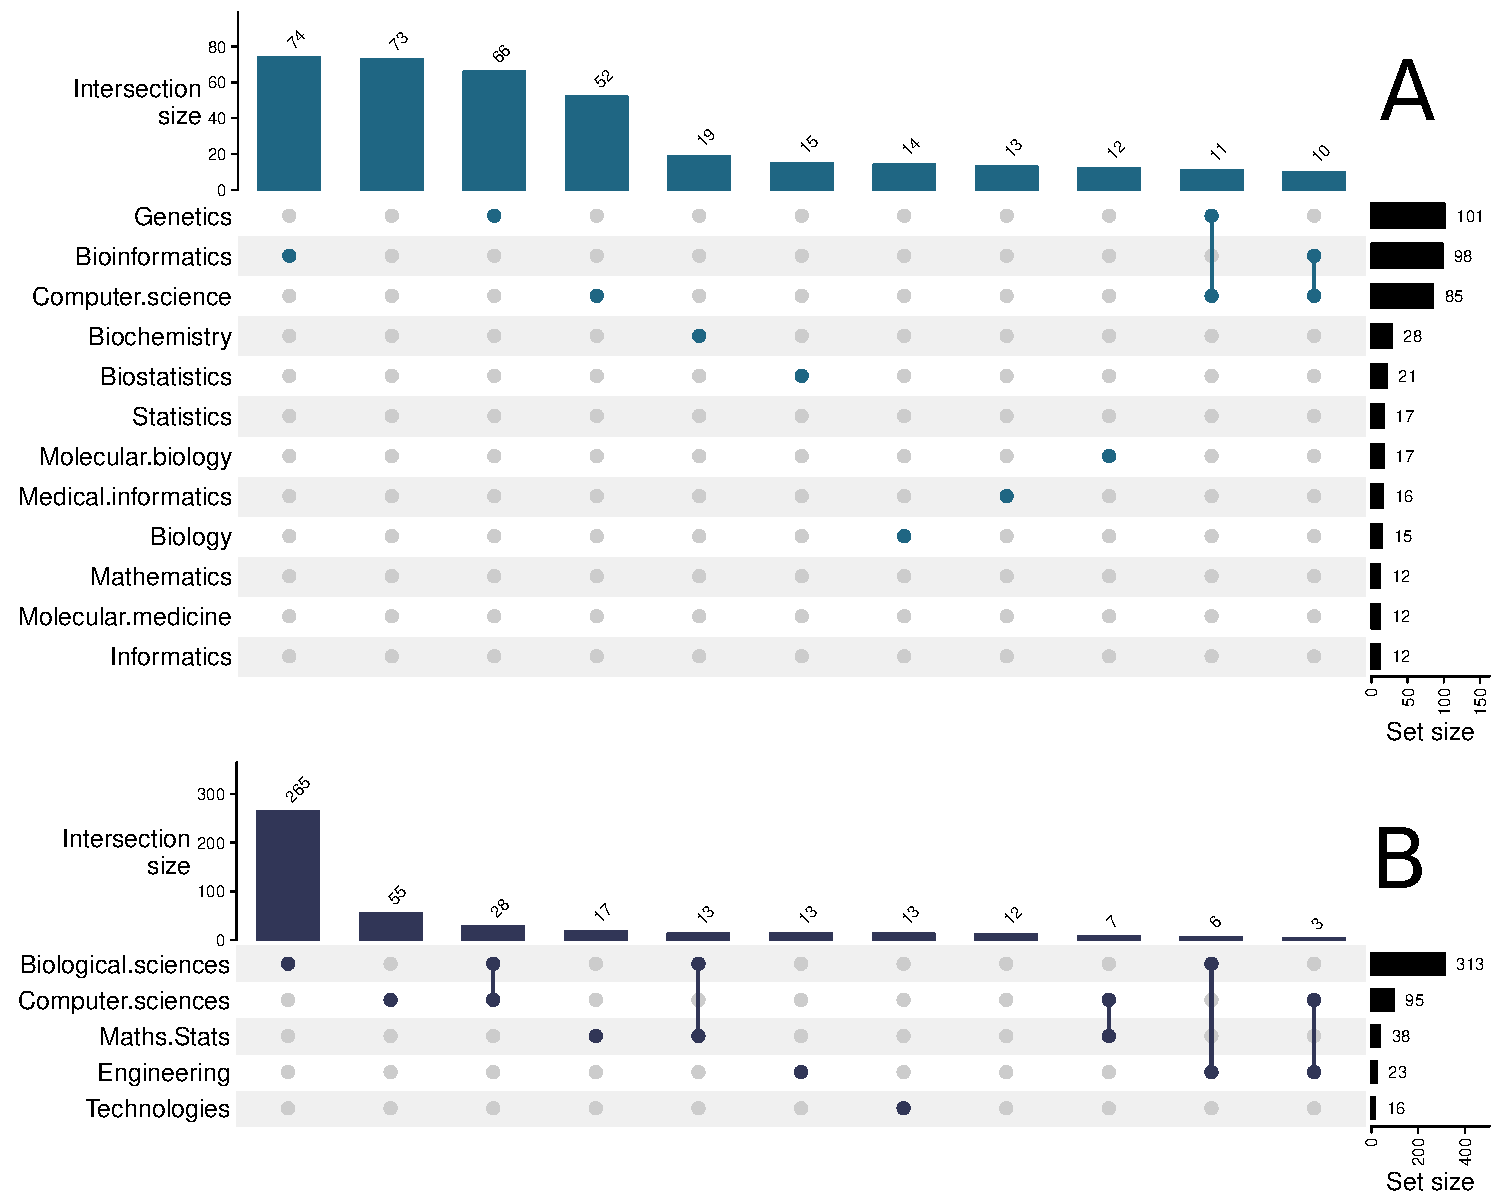
\includegraphics[width=0.6\textwidth]{upset-plots.pdf}
\end{center}
  \caption{ The number and intersection of general (\textbf{A}) or
  specific (\textbf{B}) fields that have contributed to bioinformatic
  software tools included in recent benchmark studies.  The number and
  intersection of specific fields.  }
\label{fig:fig1}
\end{figure*}


\section*{Results}

We are interested in exploring the relationship between the accuracy
of bioinformatic software tools and the academic fields of study of
their developers. Using a published corpus of accuracy rankings
for bioinformatic software tools, we mapped these tools to their
respective academic fields and evaluated how software accuracy
correlates with the developers' academic affiliations.

We obtained previously benchmarked and collated accuracy rankings from
a published supplement \cite{gardner2024}. Using these rankings, we
mapped the addresses of corresponding authors for each published
software tool to a standardized list of specific ``fields of study''
\cite{fields2014}. These fields were then grouped into higher-level
general fields and broader areas of expertise based on the address
details of each corresponding author. Figure~\ref{fig:fig1} illustrates
the number of tools representing each general and specific field. Most
bioinformatic software is developed by corresponding authors who list
Genetics, Bioinformatics, Computer Science, or similar departments as
their primary address (Figure~\ref{fig:fig1}A). Among the general fields,
the Biological Sciences produce the most software tools, followed by
the Computer Sciences (Figure~\ref{fig:fig1}B).

\begin{figure*}[ht!]
\begin{center}
  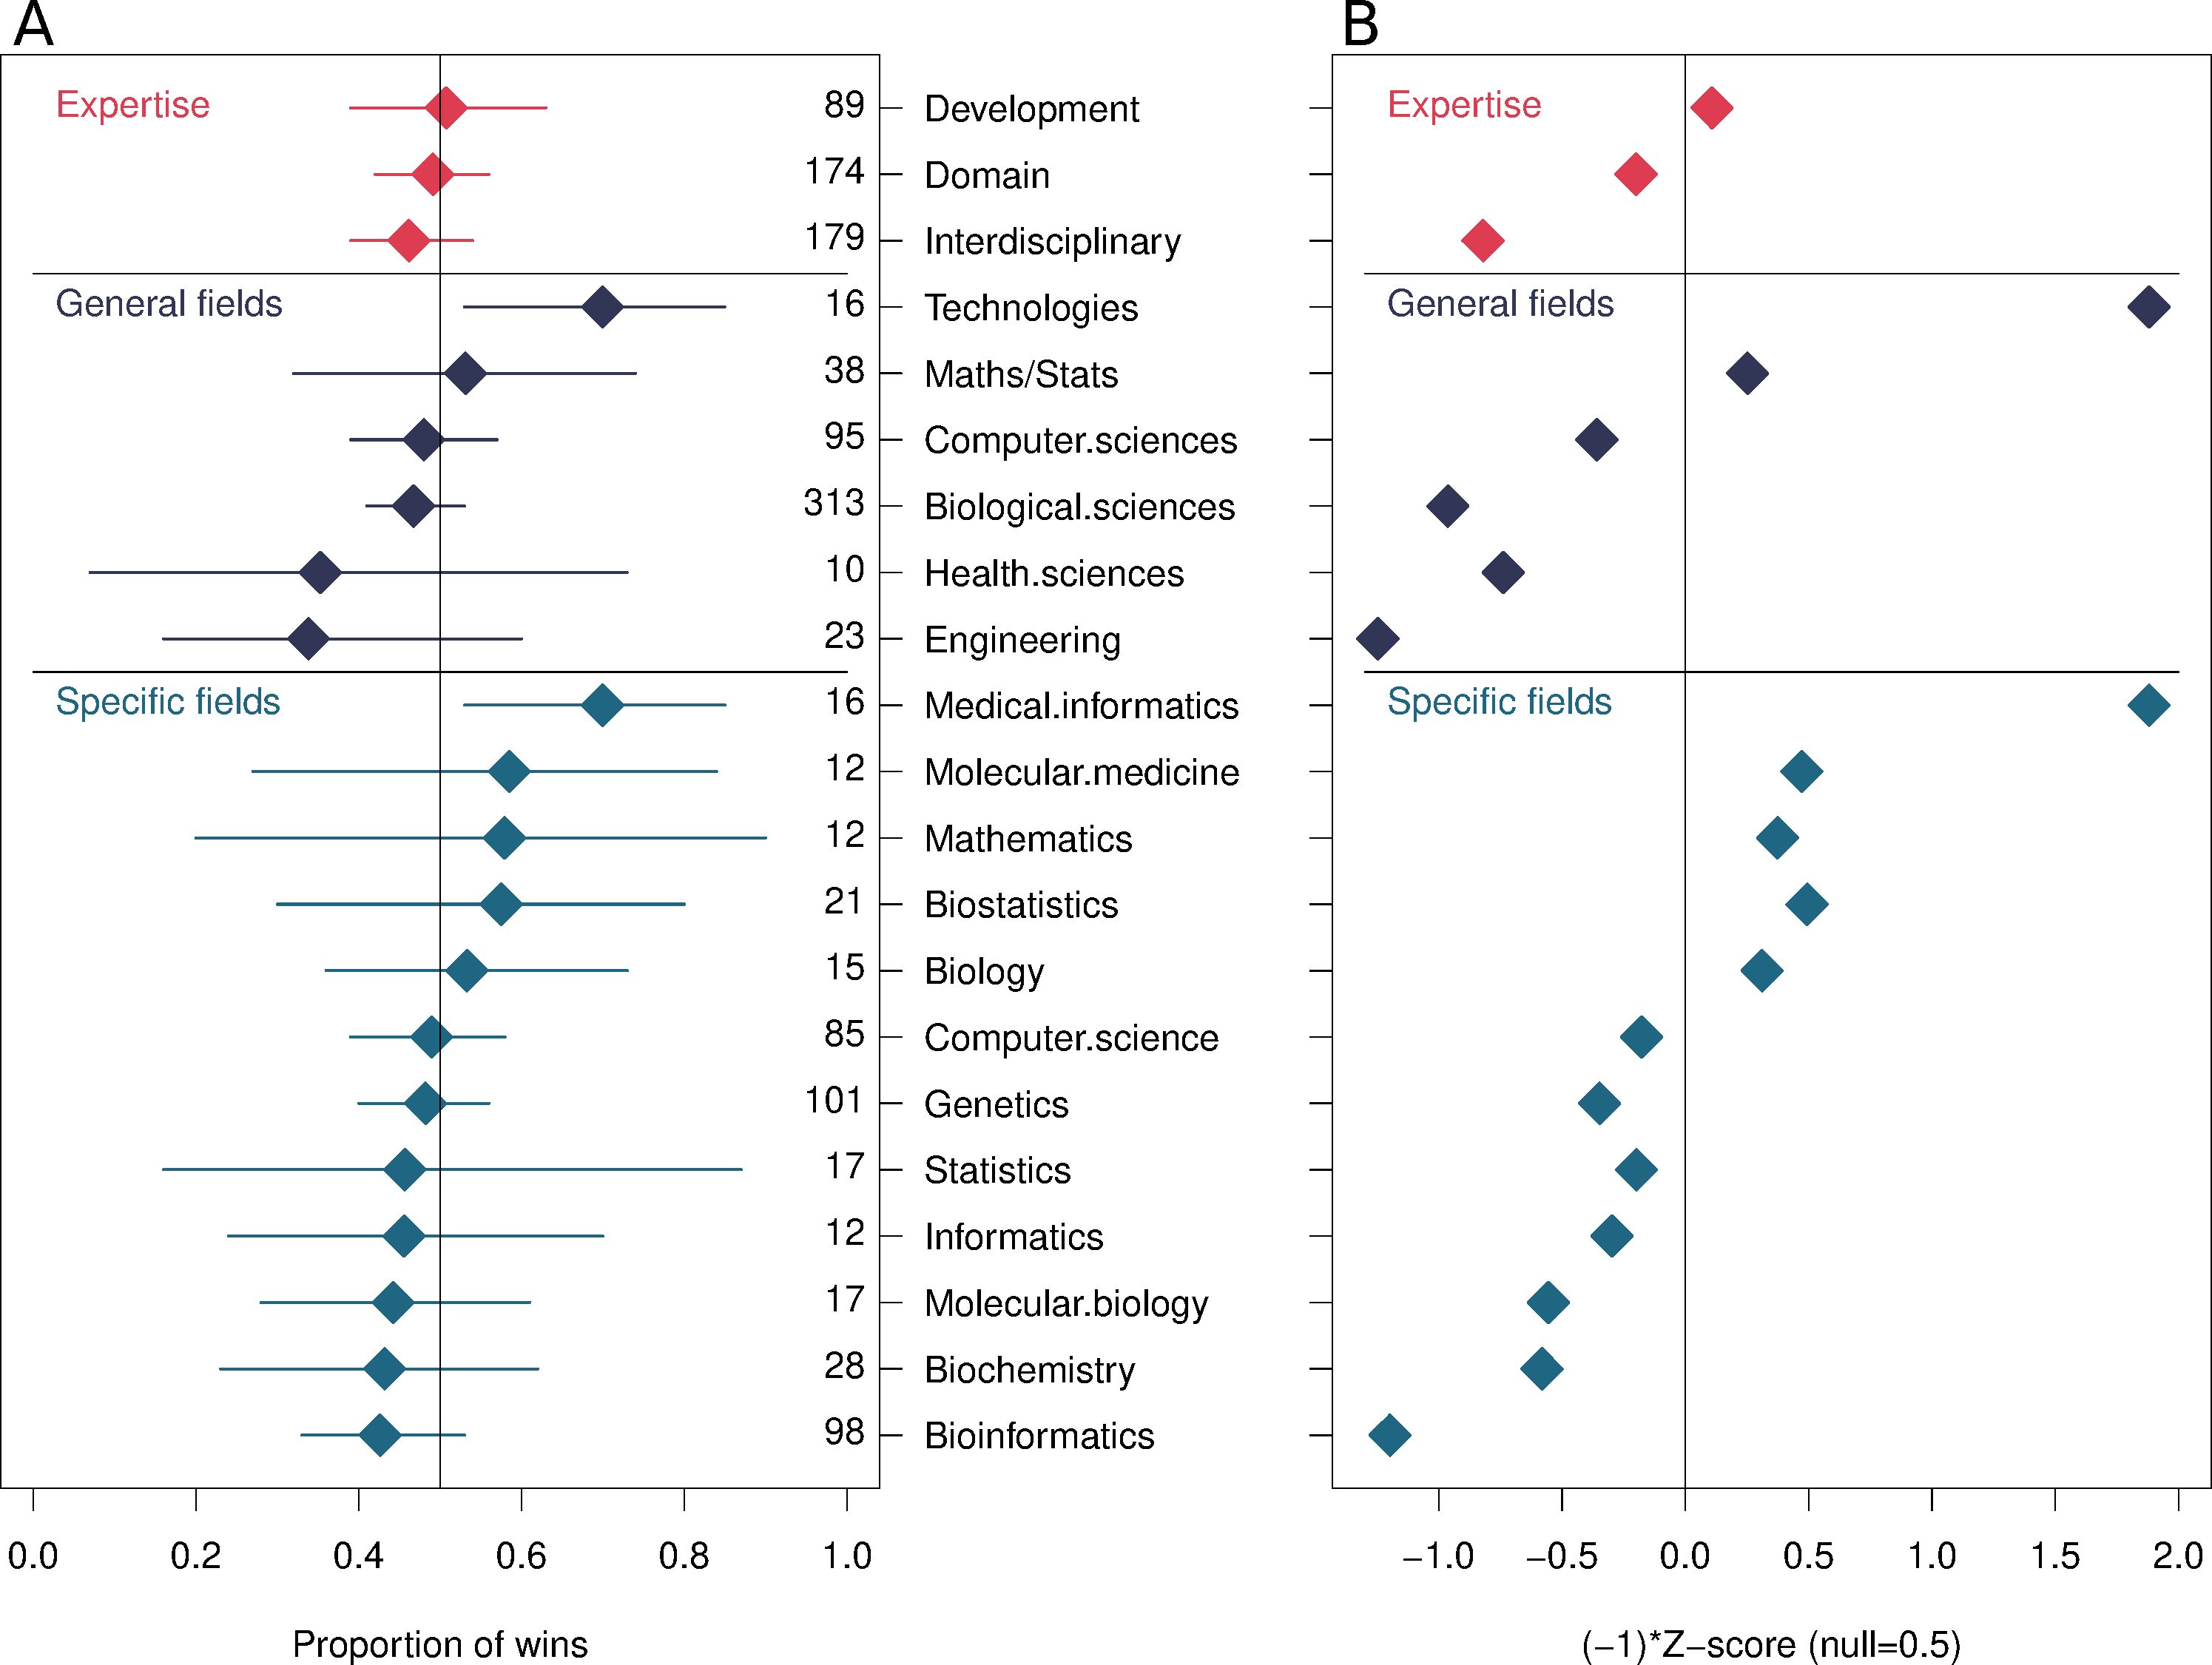
\includegraphics[width=0.8\textwidth]{forest-z-Plot.pdf}
\end{center}
\caption{(\textbf{A}) A forest plot, illustrating the mean and 95\%
  confidence intervals of the proportion of times software tools
  published by a given field ``win'' in pairwise
  comparisons. Confidence intervals and the mean was determined using
  a bootstrapping procedure. Within each field the entries have been
  sorted by the mean number of wins. The sample size for each field is
  indicated by the column of numbers on the right of the figure.
  (\textbf{B}) A Z-score was computed for each distribution of
  bootstrap samples for each field. The expected proportion of wins
  for randomly selected groups of tools was used as ``$x$''
  (i.e. null=0.5).}
\label{fig:fig2}
\end{figure*}

The mean proportion of wins (e.g., if tool `A' outranks tool `B', this
counts as a win for tool `A') and the corresponding Z-scores provide a
method to rank fields of study based on the relative accuracy of
bioinformatic software benchmarked between 2005 and 2020, compared to
the expected number of wins for random groupings (i.e., $wins =
0.5$). A higher proportion of wins and a greater $(-1) * Z-score$
indicate that tools from a particular department more frequently
outperformed competing tools in independent benchmarks.

The specific and general field that outperformed all others is
``Medical Informatics'', a branch of ``Technologies'', with 16
software tools categorized under both fields. Among these, five are
different parameter options for the MAFFT multiple sequence alignment
tool \cite{katoh2008recent}.  These Medical Informatic tools have a mean proportion of wins of
0.70 and 95\% confidence interval of $0.53-0.85$, which excludes the
null value of 0.5. The corresponding Z-score is $-1.88$, and after correcting for multiple testing, the P-value is $0.29$.

At the other end of the spectrum is ``Bioinformatics''. Ironically,
authors that list ``Bioinformatics'' in their address field tend to
produce less accurate software for bioinformatic applications. The
mean proportion of wins was 0.43, with a 95\% confidence interval of
$0.33-0.53$. The corresponding Z-score is $1.20$ and after correcting
for multiple testing the P-value is $0.46$.


The general field of ``Engineering'' also ranked low, with a mean
proportion of wins of just 0.34 and a 95\% confidence interval of
$0.16-0.60$. The corresponding Z-score is $1.25$. This general field
comprises several smaller specific fields, such as "Bioengineering and
Biomedical Engineering," "Computer Engineering," and "Electrical and
Electronics Engineering." However, since none of these specific fields
individually had more than ten corresponding software tools, they were
excluded from the more detailed analysis.

The remaining general and specific academic fields have confidence
intervals that include the null value of 0.5, and relatively modest
Z-scores that range from -0.49 to 0.96. The P-values for each were
greater than $0.05$. 

For the highest level field classifications of software development
expert, biological domain expert or interdisciplinary expert each had
similar mean proportions of wins (0.51, 0.49 and 0.46
respectively). The interdisciplinary experts had a lower Z-score of
$-0.87$, which corresponds to $P=0.46$ after correcting for multiple
testing.

%followed by ``Molecular Medicine''
%We have deliberately not computed P-values or other measures of
%significance for this study. 

\section*{Conclusions and Limitations}

We tested the assumption that the speciality of academic departments
reflect the quality of the research software they produce. Our
findings showed no significant association, after correcting for
multiple-testing, between the type of academic expertise -- whether
biological domain expert, software developer, or interdisciplinary
scientist -- and the accuracy rankings of bioinformatic software
tools. This leads us to conclude that assumptions linking academic
department affiliation to the quality of bioinformatic software are
likely incorrect. Similarly, both general and specific research fields
showed no significant associations (Figure~\ref{fig:fig2}).

Our earlier paper found that a long-term commitment to keeping
software updated was the primary factor associated with accurate
software tools. This current study complements that finding by demonstrating 
that citation metrics (e.g. journal impact factors and
author H-index), tool age, tool speed, and now academic fields of
inquiry are \textbf{not} associated with software accuracy.

We focus on software tool accuracy here \cite{weber2019essential}. While speed, usability and
some features of software tools are important, in our opinion the
primary concern for bioinformatic software tools is the accuracy of
the results they produce. As poor predictions may have long-term consequences for
our general research field. 

Medical Informatics, under the broader category of "Technologies," is
identified as the top-performing group in developing accurate
bioinformatic software tools. The tools include a number of methods
for structural variation detection, single-cell profiling, long-read
assembly, multiple sequence alignment and are derived from several
different research teams. 

Bioinformatics and Engineering ranked lower in terms of software
accuracy. Tools developed by authors who affiliated with
"Bioinformatics" typically had slightly lower accuracy than that of
other fields. However, this was not a statistically significant
finding. In addition (further bad news for this author),
``Biochemistry'' was similarly ranked, again this was not a
statistically significant finding.

This leads us to conclude that an individual's host department are not
reflective of the quality of software that they are capable of
producing ($p>0.05$ in all instances). As a consequence, the academic
department should not be used as a proxy for judging the potential of
software development projects.

\textbf{Limitations:} Some benchmarks rank multiple tool options,
which can introduce modest to large effects as these options may not
be independent. Additionally, the accuracy metrics used are diverse,
and some may be flawed under certain conditions; for example,
``accuracy'' can be misleading with large class-imbalances
\cite{luque2019impact}, and the N50 metric for sequence assembly has
been criticized by some commentators \cite{xie2021pdr}. Moreover, some
benchmarks are relatively small, so even small changes in rank can
have a substantial impact on the proportion of wins for intermediate
rankings. Lastly, the cohort of benchmarks has not been updated to
include more recent results.

There is often a disconnect between a bioinformatic tool developer's
training and their host department. For example, the author of this
study completed an undergraduate degree in mathematics, a PhD in
bioinformatics, postdoctoral fellowships in computer science and
molecular biology departments, worked for several years at a genomics
research institute, and is currently employed in a Biochemistry
Department. The ``Biochemistry'' departmental label does not accurately
reflect the author's training or recent publications. In fact, the
author admits to not recalling key details of glycolysis, the citric
acid cycle, or the structures of amino acids and proteins.

The last, or corresponding, author is typically the principal
investigator who leads a project. They may have limited direct
involvement in the development of any software tool, while
their role is mainly to provide resources and overall direction for
the project. However, there is likely to be a significant overlap between the
department of the first author, who is usually the primary developer
of the tool, and the department of the last author (though this was
not tested in this study). Therefore, we expect that the results will
be broadly similar if first-author departments were analyzed instead.


%Open questions: what impact does training have on improving software quality?
%We could end with echoing the call for more training and a continued 
%e.g. \cite{johanson2018software,siepel2019challenges}

\section*{Methods}

~~~~\textbf{Pre-registration:} This study's desired sample size, included variables, hypotheses, and
planned analyses were pre-registered on the Open Science Framework
%(https://doi.org/10.17605/OSF.IO/92PTZ)
prior to any unpublished data being collected \cite{gardner2024}.

\textbf{Benchmarking data:} software ranks from previously gathered
benchmarks are publically available \cite{Gardner:2022}, these include data from
68 publications that rank the accuracy of different sets of 498
distinct software tools.

%The methodology section should provide more detail about how the software tools were selected and mapped to academic fields. It’s important to describe how biases or inconsistencies in mapping were addressed.
\textbf{Mapping tools to academic field:} For each software tool, the
corresponding publication(s) were identified, and the addresses of the
primary corresponding author were manually extracted when
available. If an author listed multiple addresses, only the first two
were used. In cases with multiple corresponding authors, the last
corresponding author was chosen.

The department names of the authors were mapped to the closest
associated ``fields of study'' as defined by the National Science
Foundation \cite{fields2014}. We analysed these fields at three
hierarchical levels: first, specific fields (e.g. ``genetics'',
``computer science'', ``bioinformatics'' etc), which were then mapped
to broader general fields (e.g. ``biological sciences'', ``computer
sciences'' etc). Thirdly, we categorized them into three types of
expertise: \textbf{development experts}, \textbf{domain experts} and
\textbf{interdisciplinary experts}.  Development experts, from fields
such as computer science, mathematics, and engineering, are expected
to bring relevant expertise in software engineering and the
mathematical modeling of biological problems. Domain experts, from the
biological and health sciences, are anticipated to possess detailed
knowledge of their subject area and to be invested in producing
high-performing software for their research needs. Interdisciplinary
experts come from fields such as bioinformatics, biostatistics, and
biomathematics, and also include researchers who list both development
and domain expertise (e.g. ``Computer Science'' and ``Genetics''). We
have treated some fields as synonymous; for example, ``Computational
Biology'' was mapped to ``Bioinformatics'', and ``Genomics'' is mapped
to ``Genetics''.

We restricted all subsequent analyses to fields that contain at least 10
software tools in our benchmark corpus. This mitigated against
potential issues due to small sample sizes. 

\textbf{Statistical analysis:} The accuracy data is derived from
benchmarks using a diverse number of metrics that include sensitivity,
specificity, PPV, FDR, error rates, AUROC, MCC and others
\cite{weber2019essential}. The number of tools ranked in any benchmark
ranged from 3 to 50. In order to obtain a representative measure of
accuracy for a field that accounts for the diversity in accuracy measures and
number of ranked tools, we employed a rank-based and
bootstrapping strategy.
We randomly sampled, with replacement, sets of 200 tools from the total of 498 tools. For each tool, a corresponding benchmark was selected at random, and the number of times the tool ``won'' against another tool was recorded, along with the total number of pairwise comparisons made. These counts of wins and total comparisons were then assigned to the corresponding specific, general, and expertise areas. This process was repeated 1,000 times to estimate the mean proportions of wins for each field, along with a 95\% confidence interval for these values (Figure~\ref{fig:fig2}A).
Additionally, we calculated a Z-score for each field to determine the number of standard deviations the mean number of wins deviates from the expected null value of 0.5 for randomly grouped tools
(Figure~\ref{fig:fig2}B).

$Z-score=\frac{x-\mu}{\sigma}$

Where $\mu$ is the mean, $\sigma$ is the standard deviation, $x$ is the raw
value. In this case we set $x=0.5$ as this is the null expectation for
the proportion of wins for randomly grouped sets of tools. For the
purposes of illustration we plot $(-1)*z$ so that the direction is the
same as for the ``proportion of wins'' forest plot
(Figure~\ref{fig:fig1}). 

P-values are computed from the absolute value of the Z-scores to
evaluate if any field is significantly distinguished from the null
i.e. $P[X > x]$. The P-values are corrected for multiple testing by
controlling the false discovery rate method
\cite{benjamini1995controlling}.


\noindent\textbf{Data and analysis scripts availability}

The data, scripts, figures and manuscript draft files are availble at the GitHub repository:\\
\href{https://github.com/ppgardne/departments-software-accuracy}{https://github.com/ppgardne/departments-software-accuracy}

\noindent\textbf{Funding:} This research was supported by the MBIE data
science platform ``Beyond Prediction: explanatory and transparent data
science'', Genomics Aotearoa, and Marsden
Grants 19-UOO-040 and 20-UOA-282.

\noindent\textbf{Authors' contributions:} this work was conceived by 
PPG, designed by PPG, the analysis was carried out by PPG, interpretation of the results was by PPG,
the manuscript was drafted by  PPG.
All authors revised and edited the final manuscript. All authors approve the submitted version. 

%----------------------------------------------------------------------------------------
%       REFERENCE LIST
%----------------------------------------------------------------------------------------
\bibliographystyle{unsrt}
\bibliography{references.bib}


\end{document}
